% ---------------------------------------------------------------------------------------------------------
% 問題設定・記法
% ---------------------------------------------------------------------------------------------------------
\section{問題設定}
\label{sec:problem}
\subsection{装置と座標系}
クリフディメンションは向かい合う 2 枚の壁からなる（図~\ref{fig:device3d}）．
クリフ A は上下に，クリフ B は左右に動き，それぞれの壁の前面に奥行き 3\,cm の突起が水平に走っている．
挑戦者は A の突起に両手でぶら下がり，体を振って離手し，空中で体の向きを変えて B の突起を両手で掴む．
本稿は矢状面（体を横から見た面）の運動を扱い，A から B へ向かう水平方向を $+x$，鉛直上向きを $+y$ とし，
B の突起の上面（把持面）の高さを $y=0$ に置く．
\begin{figure*}[t]
\centering
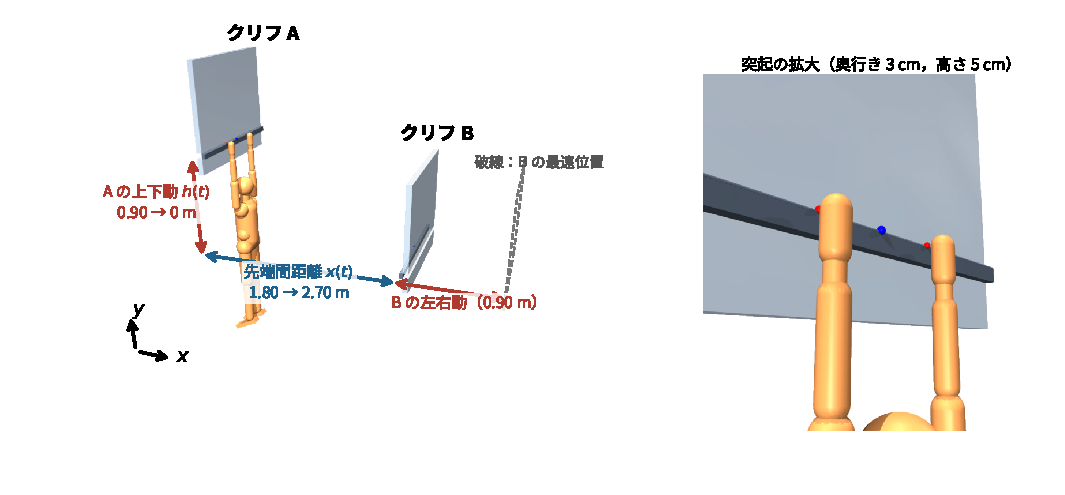
\includegraphics[width=\linewidth]{../results/figs/device3d.pdf}
\caption{装置の 3 次元図（左）と突起の拡大（右）．クリフ A は上下に 0.90\,m，クリフ B は左右に 0.90\,m 動く．
図は装置位相 $\phi=0$（A が最も高く，B が最も近い）で，挑戦者が A にぶら下がった開始姿勢を示す．
$x$ は A から B へ向かう水平方向，$y$ は鉛直上向きで，B の把持面の高さを $y=0$ とする．
人体は第~\ref{sec:spatial}節の 31 関節モデルを平面モデルの姿勢に合わせて描画したものである．}
\label{fig:device3d}
\end{figure*}

装置は周期 $T$ で往復する．時刻 $t$ の装置位相を $\phi=(t \bmod T)/T\in[0,1)$ と書く．
A と B の突起の先端（把持面の前縁）の位置を
\begin{equation}
\bm p_A(t)=(0,\,h(t)),\qquad \bm p_B(t)=(x(t),\,0)
\end{equation}
とし，$h(t)$ を高低差，$x(t)$ を先端間距離と呼ぶ．それぞれ
\begin{equation}
x(t)=1.80+0.90\,\rho_\epsilon(\phi),\qquad h(t)=0.90\,\bigl(1-\rho_\epsilon(\phi)\bigr)\quad[\mathrm{m}]
\end{equation}
である．$\rho_\epsilon(\phi)\in[0,1]$ は 0 から 1 へ上がって 0 へ戻る三角波を，折り返しの前後 $\epsilon=0.20$\,s だけ
滑らかにつないだ進行関数で，折り返し点で装置速度が 0 になる（図~\ref{fig:device}）．
$\phi<0.5$ を\textbf{往路}（A が下がり B が遠ざかる），$\phi\ge0.5$ を\textbf{復路}（A が上がり B が近づく）と呼ぶ．
A が最も高いのは B が最も近いとき（$\phi=0$）である．
\begin{figure}[t]
\centering
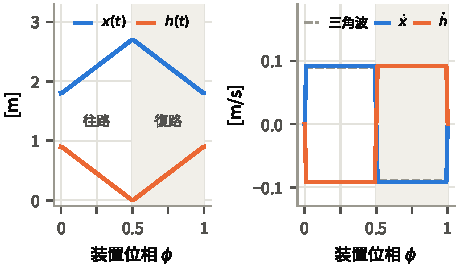
\includegraphics[width=\linewidth]{../results/figs/device_motion.pdf}
\caption{装置運動（$T=20$\,s の例）．左：先端間距離 $x(t)$ と高低差 $h(t)$．右：装置速度．
破線は滑らかにする前の三角波で，本稿は実線の平滑化した運動を用いる．}
\label{fig:device}
\end{figure}

\subsection{突起形状と成功条件}
突起は壁の前面から 3\,cm 張り出し，鉛直方向の高さは 5\,cm である（図~\ref{fig:schematic} 右）．
突起の下 15\,cm は壁の本体前面で，手首と前腕の動きを制限する．それより下は何もない開放空間で，体は壁の下をくぐれる．
先端の上縁には手への食い込みを避ける半径 5\,mm の丸みを与えた．
挑戦者は A を両手で把持し，胸を A に向けて静止した状態から始める．
1 周期 $T$ 以内に離手し，B を両手で捕捉して，そのまま 2.0\,s 保持できれば成功とする．

\subsection{把持負荷の単位：$\Fref$ と $\Fmax$}
成否を決めるのは，突起が両手に及ぼす反力 $\bm R=(R_x,R_y)$ の大きさが指の把持容量に収まるかどうかである．
本稿は二つの力を区別する．
$\Fref=1300$\,N は\textbf{表示の単位}であり，把持利用率
\begin{equation}
U(t)=\frac{\|\bm R(t)\|}{\Fref},\qquad \Upk=\max_t U(t)
\end{equation}
を定義するためだけに使う．$\Upk$ は「その動作に必要な両手の把持容量が $\Fref$ の何倍か」を表し，
$\Upk\times1300$\,N が必要把持容量である．体重比で述べるときは BW（$=mg$，$g=9.81$\,m/s$^2$）を単位にする．
一方 $\Fmax$ は，閉ループ評価で挑戦者に\textbf{実際に許す}把持容量であり，全手法で同じ値を使う．
ネットワークの予測によって $\Fmax$ が引き上げられることはない．
閉ループの成功率は $\Fmax/\Fref\in\{1.0,1.25,\dots,2.5\}$ の各水準で報告し，見出しの値は $\Fmax=2\Fref=2600$\,N とする
（第~\ref{sec:protocol}節）．

\subsection{記法}
本稿で使う記号を表~\ref{tab:notation} にまとめる．平面人体モデルの記号は図~\ref{fig:schematic} に図示した．
角度はラジアン，量の上の点は時間微分，太字はベクトルを表す．星印（$J^*$ など）は最適化で得た最適値である．
\begin{figure*}[t]
\centering
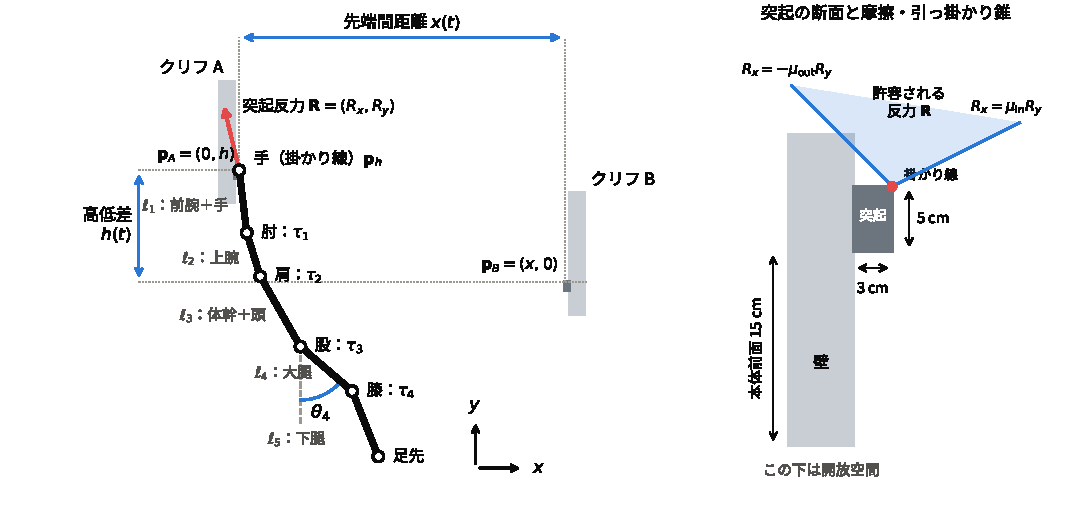
\includegraphics[width=\linewidth]{../results/figs/model_schematic.pdf}
\caption{平面 5 リンク人体モデルと記号（左），突起の断面と反力の許容範囲（右）．
各リンクの角度 $\theta_i$ は鉛直下向きから測る（図は大腿の $\theta_4$ を例示）．関節トルク $\tau_1,\dots,\tau_4$ は肘・肩・股・膝に働く．
手は突起の先端上縁の掛かり線 $\bm p_h$ に掛かり，突起から反力 $\bm R$ を受ける．
右図の青い領域は，突起が手に及ぼせる反力の範囲（摩擦・引っ掛かり錐）で，壁から離れる向きには $\mu_{\mathrm{out}}R_y$，
壁へ向かう向きには $\mu_{\mathrm{in}}R_y$ までの水平力を支えられる．}
\label{fig:schematic}
\end{figure*}
\begin{table*}[t]
\centering\scriptsize
\caption{記法．値を記したものは本稿を通じて固定した基準値である．}
\label{tab:notation}
\begin{tabular}{lp{0.345\textwidth}|lp{0.345\textwidth}}
\toprule
記号 & 意味 & 記号 & 意味 \\
\midrule
\multicolumn{2}{l|}{\textbf{装置と時間}} & \multicolumn{2}{l}{\textbf{最適化}} \\
$t$ & 時刻 [s] & $d_w,d_s,d_f$ & 待機・振り・飛行の所要時間 [s] \\
$T$ & 装置の周期 [s]（往復で 1 周期，片道 $T/2$） & $T_{\mathrm{hold}}$ & 保持時間（2.0\,s） \\
$\phi$ & 装置位相 $(t \bmod T)/T$ & $\Eeff$ & 努力指標（式~\eqref{eq:effort}） \\
$\phi_\ell,\ \phi_c$ & 離手・捕捉の瞬間の装置位相 & $J$ & 目的関数 $w_U\Upk+w_E\Eeff$ \\
$x(t),\ h(t)$ & 先端間距離，高低差 [m] & $w_U,\ w_E$ & 目的関数の重み（10，1） \\
$\rho_\epsilon(\phi)$ & 平滑化した三角波の進行関数（0〜1） & $N_S,N_F,N_H$ & 振り・飛行・保持の離散化区間数（150，30，60） \\
$\epsilon$ & 折り返しの平滑化時間（0.20\,s） & $\bm\Lambda$ & 捕捉の衝撃力積 [N\,s] \\
$\bm p_A,\ \bm p_B$ & クリフ A，B の突起先端の位置 & $\Delta_c$ & 衝撃力積を力に均す時間（50\,ms） \\
\multicolumn{2}{l|}{\textbf{人体モデル}} & $K_c,\ D_c$ & 順応捕捉の剛性・減衰（40\,kN/m，1.5\,kN\,s/m） \\
$m,\ H_b$ & 体重 [kg]，身長 [m]（基準 1.75） & \multicolumn{2}{l}{\textbf{双対変数と学習}} \\
$\ell_i$ & リンク $i$ の長さ（$i=1$：前腕＋手，2：上腕，3：体幹＋頭，4：大腿，5：下腿） & $\bm x_0,\ t_0$ & 残り最適化問題の開始状態と開始時刻 \\
$\theta_i$ & リンク $i$ の角度（鉛直下向きから） & $J^*(\bm x_0,t_0;\bm b)$ & そこから先の最適値（残りコスト） \\
$\bm p_h$ & 両手の掛かり線の位置 & $V$ & 価値．$V=J^*$ \\
$\bm q$ & 一般化座標 $(\bm p_h,\theta_1,\dots,\theta_5)$ & $\bm p^*$ & 随伴状態（costate）$\partial J^*/\partial\bm x_0$ \\
$\bm x$ & 振りの状態 $(\theta_1,\dots,\theta_5,\dot\theta_1,\dots,\dot\theta_5)$ & $\lambda_k$ & 制約 $k$ のラグランジュ乗数（影の価格） \\
$\tau_j,\ \taucap_j$ & 関節 $j$ のトルクとその上限（$j=1$：肘，2：肩，3：股，4：膝；120，160，300，240\,N\,m） & $\tgo$ & 最適な離手までの残り時間 [s] \\
$u_j$ & 正規化した指令 $\tau_j/\taucap_j\in[-1,1]$ & $U^*$ & その状態から先に必要な把持容量（$\Fref$ 比） \\
$\bm M,\bm h,\bm B,\bm J_c$ & 質量行列，重力・速度項，入力行列，手の拘束ヤコビアン & $\bm b$ & 身体・装置パラメータ（$m$，$H_b$，トルク容量の倍率，$T$） \\
\multicolumn{2}{l|}{\textbf{把持と負荷}} & $V_\vartheta,U_\vartheta,t_{\mathrm{go},\vartheta}$ & ネットワーク（パラメータ $\vartheta$）の出力 \\
$\bm R=(R_x,R_y)$ & 突起が両手に及ぼす反力 [N] & $\alpha$ & Sobolev 損失の勾配項の重み \\
$\mu_{\mathrm{out}},\ \mu_{\mathrm{in}}$ & 壁から離れる向き・壁へ向かう向きの錐の係数（1.0，2.0） & $\mathcal H$ & ハミルトニアン \\
$\Fref$ & 把持力の表示単位（1300\,N） & $T_h$ & MPC の地平（予測する時間長）[s] \\
$U(t),\ \Upk$ & 把持利用率 $\|\bm R\|/\Fref$ とその最大値 & $\rho_S$ & Spearman の順位相関係数 \\
$\Fmax$ & 閉ループ評価で実際に許す把持容量 [N] & \multicolumn{2}{l}{\textbf{閉ループ評価}} \\
BW & 体重 $mg$ を単位とする力 & $S_{c}$ & 許容容量 $\Fmax=c\,\Fref$ での成功率 \\
$v_{\mathrm{rel}}$ & 捕捉時の手と突起の相対速度 [m/s] & $\Delta S$ & 双対ラベルの有無による成功率の差 \\
 & & $\sigma_\theta,\ \sigma_{\dot\theta}$ & 開始状態に加える摂動の標準偏差 [rad]，[rad/s] \\
 & & $\delta t$ & 離手時刻の誤差 [ms] \\
 & & $\delta$ & 有限差分の刻み（正規化座標） \\
 & & $Q,\ \Delta Q$ & 候補の評価値（途中コスト＋終端価値），選択の後悔 \\
\bottomrule
\end{tabular}
\end{table*}
